\documentclass[11pt,a4paper]{report}
\usepackage[textwidth=37em,vmargin=30mm]{geometry}
\usepackage{calc,xunicode,amsmath,amssymb,paralist,enumitem,tabu,booktabs,datetime2,xeCJK,xeCJKfntef,listings}
\usepackage{tocloft,fancyhdr,tcolorbox,xcolor,graphicx,eso-pic,xltxtra,xelatexemoji}

\newcommand{\envyear}[0]{2024}
\newcommand{\envdatestr}[0]{2024-12-26}
\newcommand{\envfinaldir}[0]{webdb/2024/20241226/final}

\usepackage[hidelinks]{hyperref}
\hypersetup{
    colorlinks=false,
    pdfpagemode=FullScreen,
    pdftitle={Web Digest - \envdatestr}
}

\setlength{\cftbeforechapskip}{10pt}
\renewcommand{\cftchapfont}{\rmfamily\bfseries\large\raggedright}
\setlength{\cftbeforesecskip}{2pt}
\renewcommand{\cftsecfont}{\sffamily\small\raggedright}

\setdefaultleftmargin{2em}{2em}{1em}{1em}{1em}{1em}

\usepackage{xeCJK,xeCJKfntef}
\xeCJKsetup{PunctStyle=plain,RubberPunctSkip=false,CJKglue=\strut\hskip 0pt plus 0.1em minus 0.05em,CJKecglue=\strut\hskip 0.22em plus 0.2em}
\XeTeXlinebreaklocale "zh"
\XeTeXlinebreakskip = 0pt


\setmainfont{Brygada 1918}
\setromanfont{Brygada 1918}
\setsansfont{IBM Plex Sans}
\setmonofont{JetBrains Mono NL}
\setCJKmainfont{Noto Serif CJK SC}
\setCJKromanfont{Noto Serif CJK SC}
\setCJKsansfont{Noto Sans CJK SC}
\setCJKmonofont{Noto Sans CJK SC}

\setlength{\parindent}{0pt}
\setlength{\parskip}{8pt}
\linespread{1.15}

\lstset{
	basicstyle=\ttfamily\footnotesize,
	numbersep=5pt,
	backgroundcolor=\color{black!5},
	showspaces=false,
	showstringspaces=false,
	showtabs=false,
	tabsize=2,
	captionpos=b,
	breaklines=true,
	breakatwhitespace=true,
	breakautoindent=true,
	linewidth=\textwidth
}






\newcommand{\coverpic}[2]{
    % argv: itemurl, authorname
    Cover photo by #2~~(\href{#1}{#1})
}
\newcommand{\makeheader}[0]{
    \begin{titlepage}
        % \newgeometry{hmargin=15mm,tmargin=21mm,bmargin=12mm}
        \begin{center}
            
            \rmfamily\scshape
            \fontspec{BaskervilleF}
            \fontspec{Old Standard}
            \fontsize{59pt}{70pt}\selectfont
            WEB\hfill DIGEST
            
            \vfill
            % \vskip 30pt
            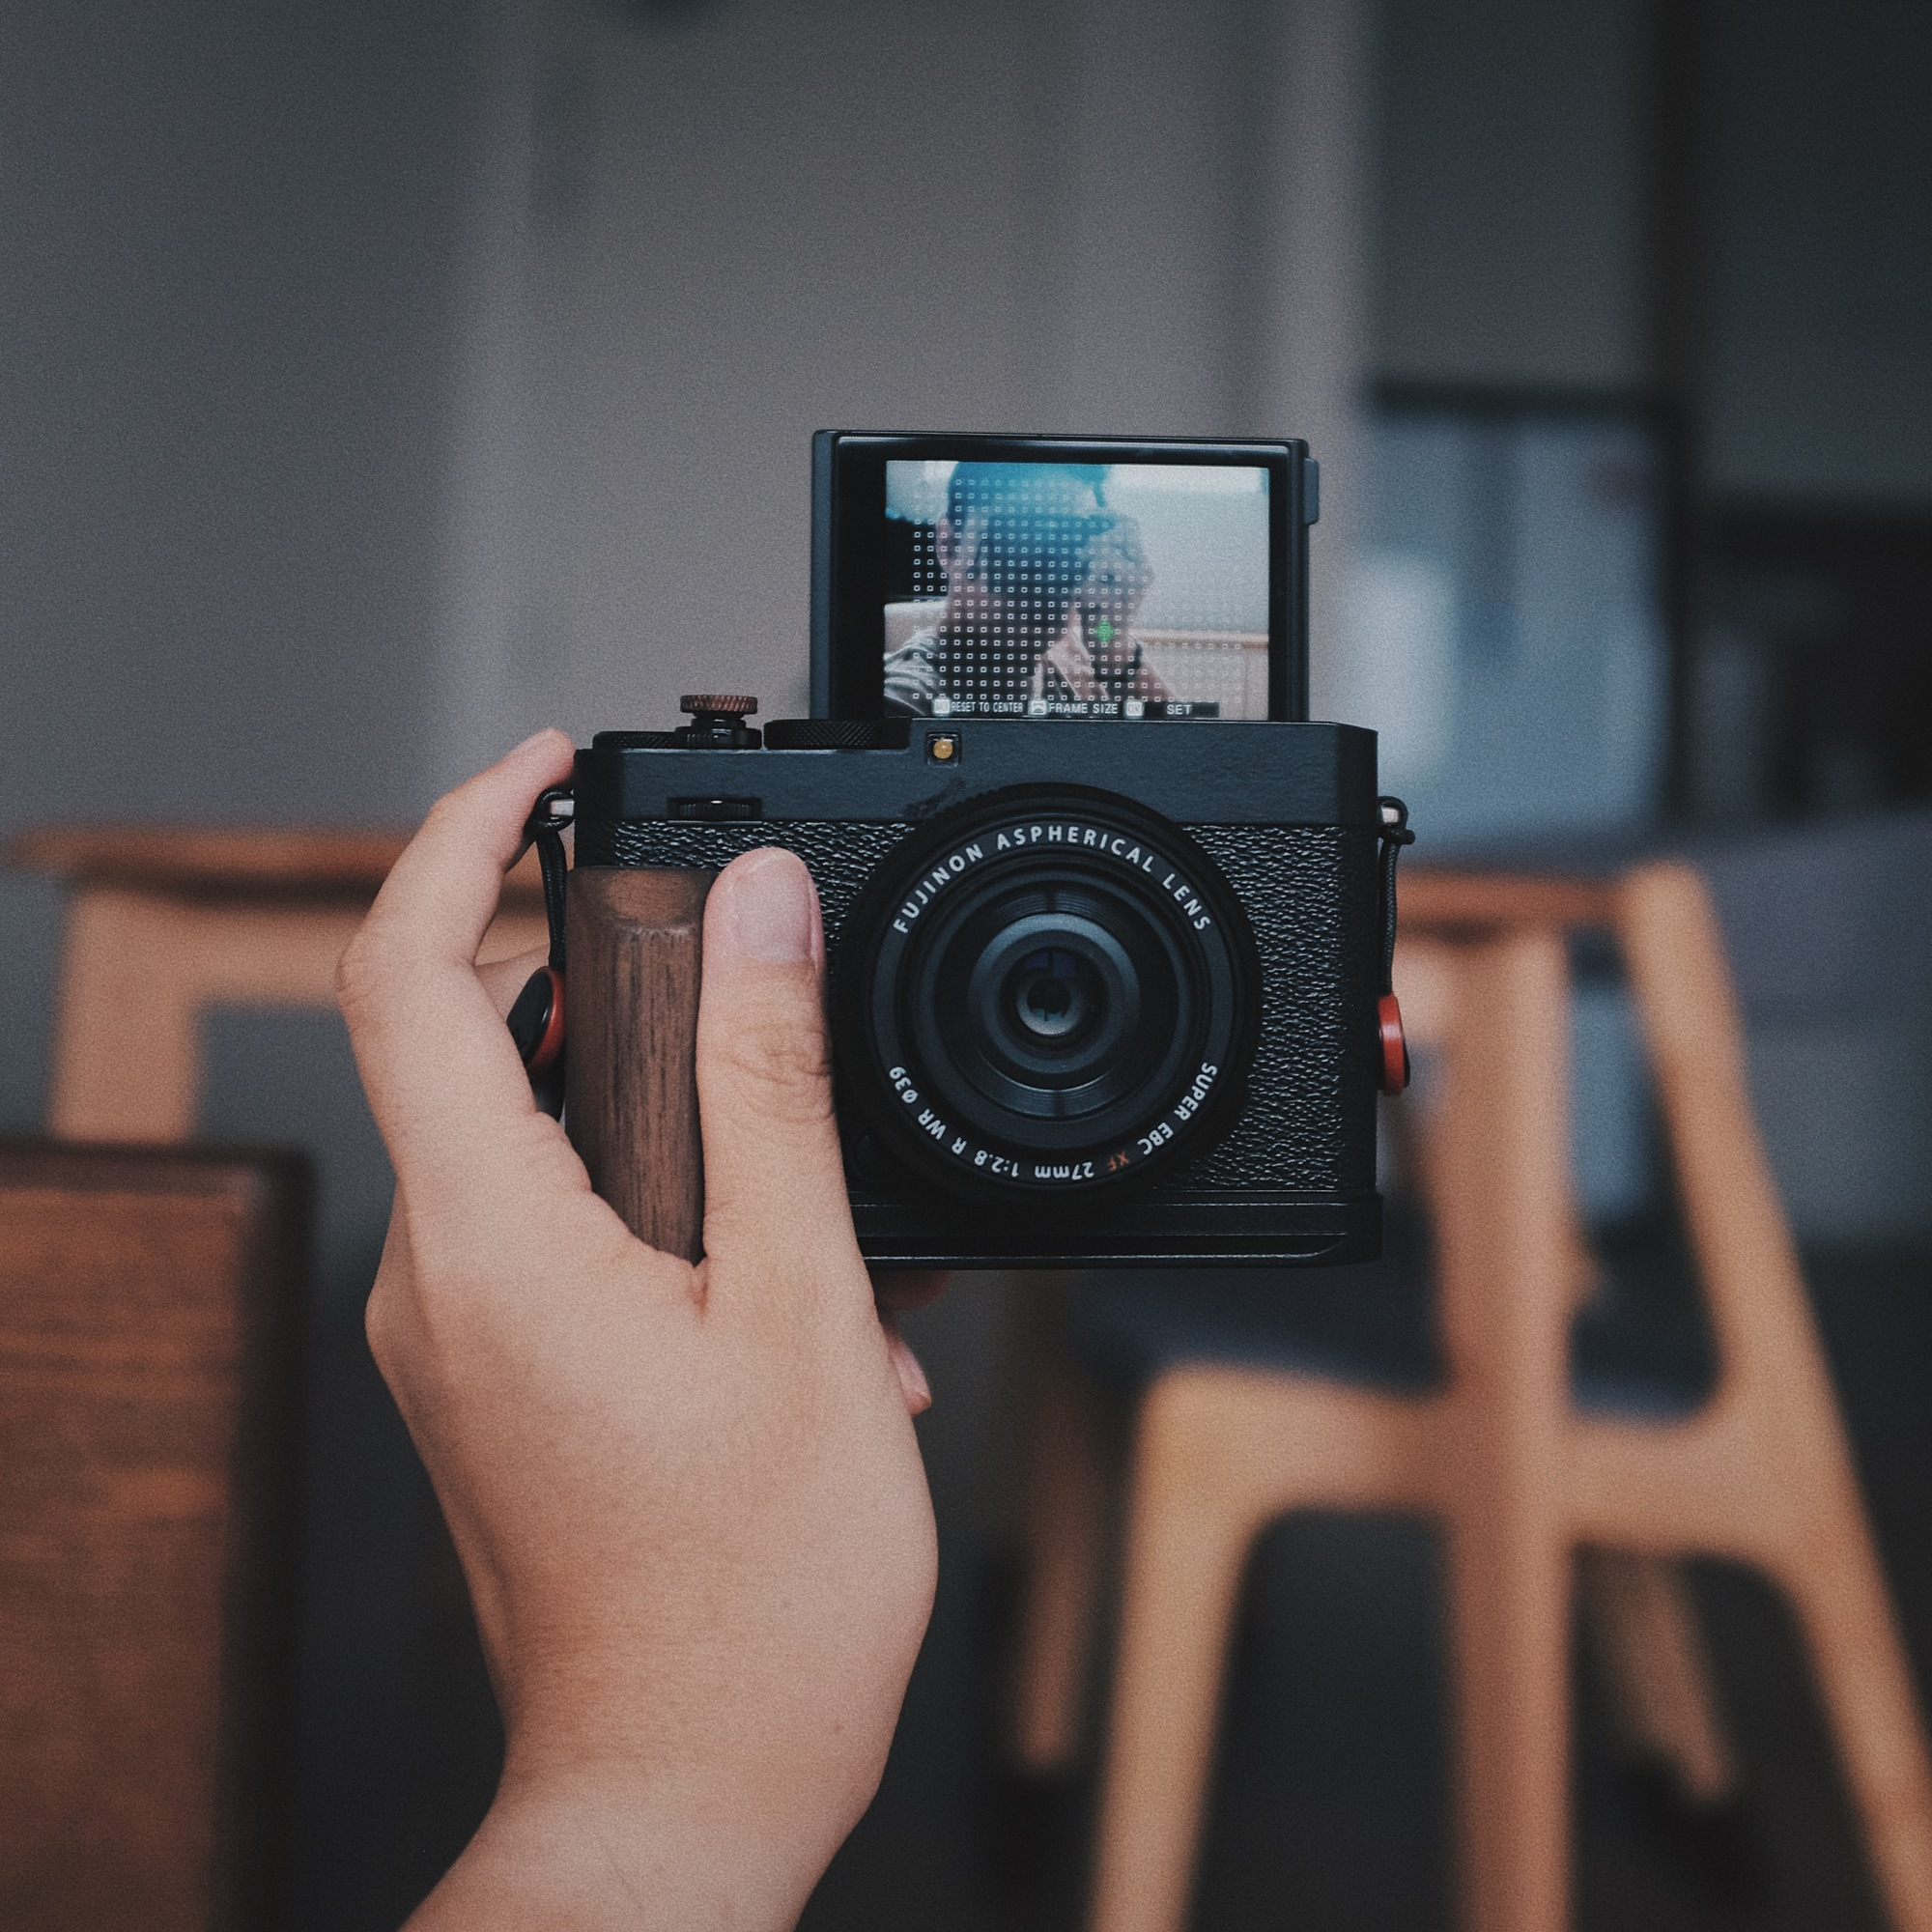
\includegraphics[width=\linewidth]{\envfinaldir/coverpic-prod.jpg}\par
            % \vskip 30pt
            \vfill

            \normalsize\rmfamily\scshape
            \copyright{} The Web Digest Project \hfill\large \envdatestr
        \end{center}
    \end{titlepage}
    % \restoregeometry
}
\newcommand{\simplehref}[1]{%
    \textcolor{blue!80!green}{\href{#1}{#1}}%
}
\renewcommand{\contentsname}{\center\Huge\sffamily\bfseries Contents\par\vskip 20pt}
\newcounter{ipartcounter}
\setcounter{ipartcounter}{0}
\newcommand{\ipart}[1]{
    % \vskip 20pt
    \clearpage
    \stepcounter{ipartcounter}
    \phantomsection
    \addcontentsline{toc}{chapter}{#1}
    % \begin{center}
    %     \Huge
    %     \sffamily\bfseries
    %     #1
    % \end{center}
    % \vskip 20pt plus 7pt
}
\newcounter{ichaptercounter}
\setcounter{ichaptercounter}{0}
\newcommand{\ichapter}[1]{
    % \vskip 20pt
    \clearpage
    \stepcounter{ichaptercounter}
    \phantomsection
    \addcontentsline{toc}{section}{\numberline{\arabic{ichaptercounter}}#1}
    \begin{center}
        \Huge
        \sffamily\bfseries
        #1
    \end{center}
    \vskip 20pt plus 7pt
}
\newcommand{\entrytitlefont}[1]{\subsection*{\raggedright\Large\sffamily\bfseries#1}}
\newcommand{\entryitemGeneric}[2]{
    % argv: title, url
    \parbox{\linewidth}{
        \entrytitlefont{#1}\par\vskip 5pt
        \footnotesize\ttfamily\mdseries
        \simplehref{#2}
    }\vskip 11pt plus 11pt minus 1pt
}
\newcommand{\entryitemGithub}[3]{
    % argv: title, url, desc
    \parbox{\linewidth}{
        \entrytitlefont{#1}\par\vskip 5pt
        \footnotesize\ttfamily\mdseries
        \simplehref{#2}\par\vskip 5pt
        \small\rmfamily\mdseries#3
    }\vskip 11pt plus 11pt minus 1pt
}
\newcommand{\entryitemAp}[3]{
    % argv: title, url, desc
    \parbox{\linewidth}{
        \entrytitlefont{#1}\par\vskip 5pt
        \footnotesize\ttfamily\mdseries
        \simplehref{#2}\par\vskip 5pt
        \small\rmfamily\mdseries#3
    }\vskip 11pt plus 11pt minus 1pt
}
\newcommand{\entryitemHackernews}[3]{
    % argv: title, hnurl, rawurl
    % \parbox{\linewidth}{
    %     \entrytitlefont{#1}\par\vskip 5pt
    %     \footnotesize\ttfamily\mdseries
    %     \simplehref{#3}\par
    %     \textcolor{black!50}{\href{#2}{#2}}
    % }\vskip 11pt plus 11pt minus 1pt
    \begin{minipage}{\linewidth}
            \entrytitlefont{#1}\par\vskip 5pt
            \footnotesize\ttfamily\mdseries
            \simplehref{#3}\par
            \textcolor{black!50}{\href{#2}{#2}}
    \end{minipage}\par\vskip 11pt plus 11pt minus 1pt
}







\begin{document}

\makeheader

\tableofcontents\clearpage




\ipart{Developers}
\ichapter{Hacker News}
\entryitemTwoLinks{Show HN: A singing synthesizer for the browser with automatic 3-part harmony}{https://news.ycombinator.com/item?id=42513276}{https://pbat.ch/recurse/demos/trio/}

\entryitemTwoLinks{Differential Growth Addon for Blender}{https://news.ycombinator.com/item?id=42513157}{https://boris.okunskiy.name/posts/blender-differential-growth}

\entryitemTwoLinks{A Minecraft server written in COBOL}{https://news.ycombinator.com/item?id=42513022}{https://github.com/meyfa/CobolCraft}

\entryitemTwoLinks{Blackcandy: Self hosted music streaming server}{https://news.ycombinator.com/item?id=42512896}{https://github.com/blackcandy-org/blackcandy}

\entryitemTwoLinks{Bird flu kills more than half the big cats at a Washington sanctuary}{https://news.ycombinator.com/item?id=42512772}{https://www.cnn.com/2024/12/25/us/bird-flu-washington-cats-cases/index.html}

\entryitemTwoLinks{Siyuan: Privacy-first, self-hosted personal knowledge management software}{https://news.ycombinator.com/item?id=42512713}{https://github.com/siyuan-note/siyuan}

\entryitemTwoLinks{Egui – An immediate mode GUI written in Rust}{https://news.ycombinator.com/item?id=42512636}{https://www.egui.rs/}

\entryitemTwoLinks{Seconds Since the Epoch}{https://news.ycombinator.com/item?id=42512371}{https://aphyr.com/posts/378-seconds-since-the-epoch}

\entryitemTwoLinks{Installing OpenWRT on an Unsupported Router}{https://news.ycombinator.com/item?id=42512050}{https://radiosocial.de/@hennichodernich/113714518196988714}

\entryitemTwoLinks{Server-Sent Events (SSE) Are Underrated}{https://news.ycombinator.com/item?id=42511318}{https://igorstechnoclub.com/server-sent-events-sse-are-underrated/}

\entryitemTwoLinks{Air missile accident emerges as probable cause of Azerbaijan E190tragedy}{https://news.ycombinator.com/item?id=42511267}{https://www.euronews.com/2024/12/25/azerbaijani-passenger-plane-crashes-near-kazakh-city-of-aktau}

\entryitemTwoLinks{I thought I found a bug}{https://news.ycombinator.com/item?id=42510776}{https://www.os2museum.com/wp/i-thought-i-found-a-bug/}

\entryitemTwoLinks{Into CPS, Never to Return}{https://news.ycombinator.com/item?id=42510696}{https://bernsteinbear.com/blog/cps/}

\entryitemTwoLinks{Portspoof: Emulate a valid service on all 65535 TCP ports}{https://news.ycombinator.com/item?id=42509953}{https://github.com/drk1wi/portspoof}

\entryitemTwoLinks{Sherlock: Hunt down social media accounts by username across 400 social networks}{https://news.ycombinator.com/item?id=42509809}{https://sherlockproject.xyz/}

\entryitemTwoLinks{Ask HN: Resources for general purpose GPU development on Apple's M* chips?}{https://news.ycombinator.com/item?id=42509730}{https://news.ycombinator.com/item?id=42509730}

\entryitemTwoLinks{Three-quarters of the land is drying out, 'redefining life on Earth'}{https://news.ycombinator.com/item?id=42509434}{https://grist.org/international/three-quarters-of-the-worlds-land-is-drying-out-redefining-life-on-earth/}

\entryitemTwoLinks{Ask HN: What skills do you want to develop or improve in 2025?}{https://news.ycombinator.com/item?id=42509408}{https://news.ycombinator.com/item?id=42509408}

\entryitemTwoLinks{F*: A proof oriented general purpose programming language}{https://news.ycombinator.com/item?id=42508642}{https://fstar-lang.org/}

\entryitemTwoLinks{Ruby 3.4.0}{https://news.ycombinator.com/item?id=42507312}{https://www.ruby-lang.org/en/news/2024/12/25/ruby-3-4-0-released/}\ichapter{Phoronix}
\entryitemGeneric{\hskip 0pt{}KDE Enjoyed A Stellar 2024 With The Debut Of The Plasma 6 Desktop}{https://www.phoronix.com/news/KDE-2024-Highlights}

\entryitemGeneric{\hskip 0pt{}The Performance Benefits Of Linux 6.12 LTS Over Linux 6.6 LTS}{https://www.phoronix.com/review/linux-66-612-lts}

\entryitemGeneric{\hskip 0pt{}Intel Linux Performance Optimizations \& Intel's Other Open-Source Wins From 2024}{https://www.phoronix.com/news/Intel-Linux-Open-Source-2024}

\entryitemGeneric{\hskip 0pt{}AMD Ryzen PCs May See More Power Savings Out-Of-The-Box With Linux 6.14}{https://www.phoronix.com/news/AMD-P-State-Ryzen-Linux-6.14}

\entryitemGeneric{\hskip 0pt{}Reiser5 Would Be Turning Five Years Old But Remains Dead}{https://www.phoronix.com/news/Reiser5-Five-Years-Old}

\entryitemGeneric{\hskip 0pt{}Pre-Content fanotify / fanotify Hierarchical Storage Management Expected For Linux 6.14}{https://www.phoronix.com/news/Linux-6.14-precontent-fanotify}

\entryitemGeneric{\hskip 0pt{}Hash-Based Integrity Checking Proposed For Linux To Help With Reproducible Builds}{https://www.phoronix.com/news/Hash-Based-Integrity-Linux-RB}

\entryitemGeneric{\hskip 0pt{}Linux RNDIS Removal Branch Updated For Disabling Microsoft RNDIS Protocol Drivers}{https://www.phoronix.com/news/Linux-RNDIS-Removal-EOY2024}

\entryitemGeneric{\hskip 0pt{}systemd Highlights For 2024 From Run0 To Varlink To Advancing systemd-homed}{https://www.phoronix.com/news/systemd-2024-highlights}


\ipart{Developers~~~~(zh-Hans)}
\ichapter{Solidot}
\entryitemGeneric{\hskip 0pt{}美国监狱允许囚犯远程工作}{https://www.solidot.org/story?sid=80164}

\entryitemGeneric{\hskip 0pt{}Ruby 3.4 释出}{https://www.solidot.org/story?sid=80163}

\entryitemGeneric{\hskip 0pt{}苹果解释它为什么没有构建搜索引擎的计划}{https://www.solidot.org/story?sid=80162}

\entryitemGeneric{\hskip 0pt{}中国将蝉联全球最大汽车出口国}{https://www.solidot.org/story?sid=80161}

\entryitemGeneric{\hskip 0pt{}2023 年德国生育率降至超低}{https://www.solidot.org/story?sid=80160}

\entryitemGeneric{\hskip 0pt{}因电力问题俄罗斯在 10 个地区禁止加密货币挖矿}{https://www.solidot.org/story?sid=80159}

\entryitemGeneric{\hskip 0pt{}猎豹的吼叫是独一无二的,能用于识别身份}{https://www.solidot.org/story?sid=80158}

\entryitemGeneric{\hskip 0pt{}日航因网络攻击导致航班延误}{https://www.solidot.org/story?sid=80157}

\entryitemGeneric{\hskip 0pt{}微软正尝试 AI 模型多元化在 Microsoft 365 Copilot 引入其它公司的模型 }{https://www.solidot.org/story?sid=80156}

\entryitemGeneric{\hskip 0pt{}Google 合同工被要求对比 Gemini AI 和 Claude 的结果}{https://www.solidot.org/story?sid=80155}

\entryitemGeneric{\hskip 0pt{}微软称 Edge 用户过去一年完成了百亿次 AI 聊天 }{https://www.solidot.org/story?sid=80154}

\entryitemGeneric{\hskip 0pt{}伊朗解除对 WhatsApp 和 Google Play 的封禁}{https://www.solidot.org/story?sid=80153}

\entryitemGeneric{\hskip 0pt{}中国黑客被指操控 Androxgh0st 僵尸网络 }{https://www.solidot.org/story?sid=80152}

\entryitemGeneric{\hskip 0pt{}苹果通过租用云端英伟达 GPU 避免与该公司打交道}{https://www.solidot.org/story?sid=80151}

\entryitemGeneric{\hskip 0pt{}为 Meta 审核内容的肯尼亚人被诊断有严重 PTSD}{https://www.solidot.org/story?sid=80150}

\entryitemGeneric{\hskip 0pt{}美中通过犯罪查获拥有大量比特币}{https://www.solidot.org/story?sid=80149}

\entryitemGeneric{\hskip 0pt{}朝鲜黑客窃取了价值 13.4 亿美元的加密货币}{https://www.solidot.org/story?sid=80148}

\entryitemGeneric{\hskip 0pt{}巴西以奴隶劳工为由下令比亚迪工厂停建}{https://www.solidot.org/story?sid=80147}

\entryitemGeneric{\hskip 0pt{}华硕圣诞节给用户``惊喜''而用户以为是恶意程序}{https://www.solidot.org/story?sid=80146}

\entryitemGeneric{\hskip 0pt{}越南新法律强推实名制}{https://www.solidot.org/story?sid=80145}\ichapter{V2EX}
\entryitemGeneric{\hskip 0pt{}[推广] Fiddlebops incredibox - Where Music Meets Interactive Gaming}{https://www.v2ex.com/t/1100577}

\entryitemGeneric{\hskip 0pt{}[Local LLM] DeepSeek V3}{https://www.v2ex.com/t/1100576}

\entryitemGeneric{\hskip 0pt{}[Windows] Win11 笔记本合上盖子不到 5 分钟就休眠}{https://www.v2ex.com/t/1100574}

\entryitemGeneric{\hskip 0pt{}[程序员] 好家伙阿里云杀疯了!}{https://www.v2ex.com/t/1100573}

\entryitemGeneric{\hskip 0pt{}[Telegram] Tg 旧号改手机号}{https://www.v2ex.com/t/1100572}

\entryitemGeneric{\hskip 0pt{}[问与答] 求推荐一个移动办公的设备}{https://www.v2ex.com/t/1100571}

\entryitemGeneric{\hskip 0pt{}[硬件] 最近很火的酷态科十号充电器配 magsafe 的问题}{https://www.v2ex.com/t/1100570}

\entryitemGeneric{\hskip 0pt{}[区块链] HECO 链上资产怎么提到其他链(求大佬提供方法)(公告说 清退 HECO 链上资产了 截止 2025-01-16 号)}{https://www.v2ex.com/t/1100569}

\entryitemGeneric{\hskip 0pt{}[分享发现] 流量卡和汇丰 one 香港开卡成功分享记录/Successful Activation of a Data SIM Card and HSBC One Account in Hong Kong}{https://www.v2ex.com/t/1100568}

\entryitemGeneric{\hskip 0pt{}[生活] 看到有人抱怨送外卖不敲门}{https://www.v2ex.com/t/1100567}

\entryitemGeneric{\hskip 0pt{}[职场话题] 过来人能给毕业生一点职业规划建议吗?企业选择}{https://www.v2ex.com/t/1100565}

\entryitemGeneric{\hskip 0pt{}[ WATCH] 你们的 Apple Watch 会贴膜或者带壳么?}{https://www.v2ex.com/t/1100563}

\entryitemGeneric{\hskip 0pt{}[分享创造] 做了一個可以把 GitHub 倉庫轉成 LLM 友好提示詞 📝 的瀏覽器插件}{https://www.v2ex.com/t/1100561}

\entryitemGeneric{\hskip 0pt{}[宽带症候群] 日经贴,请问现在成都有什么流量+宽带套餐比较好的可以开吗?}{https://www.v2ex.com/t/1100560}

\entryitemGeneric{\hskip 0pt{}[iCloud] Google Photos 作为 iCloud Photos 的备份,如何解决``删除照片''不同步的问题?}{https://www.v2ex.com/t/1100559}

\entryitemGeneric{\hskip 0pt{}[问与答] 有没有方便微调各种大模型的工具}{https://www.v2ex.com/t/1100556}

\entryitemGeneric{\hskip 0pt{}[浏览器] arc 浏览器 windows 端怎么卸载的?}{https://www.v2ex.com/t/1100554}

\entryitemGeneric{\hskip 0pt{}[程序员] 近 30 年中国计算机网络考古,不知对错,希望有大佬帮我纠正}{https://www.v2ex.com/t/1100553}

\entryitemGeneric{\hskip 0pt{}[程序员] 求推荐好用免费安全的电脑控制手机的软件}{https://www.v2ex.com/t/1100551}

\entryitemGeneric{\hskip 0pt{}[程序员] QQ 被封一天我经历了什么}{https://www.v2ex.com/t/1100550}

\entryitemGeneric{\hskip 0pt{}[旅行] 西班牙七天的旅行}{https://www.v2ex.com/t/1100548}

\entryitemGeneric{\hskip 0pt{}[问与答] 注册了一个 google voice,已经拿到号码了,但为什么没有关联到我的账号}{https://www.v2ex.com/t/1100547}

\entryitemGeneric{\hskip 0pt{}[游戏主机] 遇到一个纠结的问题 二选一 买 PS5 还是 Xbox}{https://www.v2ex.com/t/1100546}

\entryitemGeneric{\hskip 0pt{}[分享发现] a16z 应用精选}{https://www.v2ex.com/t/1100545}

\entryitemGeneric{\hskip 0pt{}[Amazon Web Services] 请教 aws lightsail 怎么付款}{https://www.v2ex.com/t/1100543}

\entryitemGeneric{\hskip 0pt{}[macOS] Macos on kvm vm Linux host 共存使用环境求建议}{https://www.v2ex.com/t/1100542}

\entryitemGeneric{\hskip 0pt{}[Apple] Apple tv 上有什么优雅的去广告方式吗?}{https://www.v2ex.com/t/1100541}

\entryitemGeneric{\hskip 0pt{}[分享发现] P 站不但可以学习动作,还可以学习微积分 = = !}{https://www.v2ex.com/t/1100540}

\entryitemGeneric{\hskip 0pt{}[程序员] 避免打扰大家,晚上发一下我的产品}{https://www.v2ex.com/t/1100539}

\entryitemGeneric{\hskip 0pt{}[分享创造] 立个帖子记录下 EzPic}{https://www.v2ex.com/t/1100538}

\entryitemGeneric{\hskip 0pt{}[程序员] Python 、C\#、Node.js 有像苹果 App Store 一样每个包都经过人工审查的,可以放心随便安装包的安全仓库吗?}{https://www.v2ex.com/t/1100537}

\entryitemGeneric{\hskip 0pt{}[分享创造] 给首页导航增加了 chrome 书签导出导入功能~最强 AI 编辑器 Cursor 辅助完成!}{https://www.v2ex.com/t/1100536}

\entryitemGeneric{\hskip 0pt{}[macOS] kvm 虚拟黑苹果后,求键盘和触板推荐}{https://www.v2ex.com/t/1100534}

\entryitemGeneric{\hskip 0pt{}[分享发现] Edge 终于支持收藏夹排序了!}{https://www.v2ex.com/t/1100533}

\entryitemGeneric{\hskip 0pt{}[宽带症候群] 公网 ip 不是随机分配的吗}{https://www.v2ex.com/t/1100532}

\entryitemGeneric{\hskip 0pt{}[问与答] [紧急]服务器到期,有适合搭建回国 WireGuard 的云服务器吗?}{https://www.v2ex.com/t/1100531}

\entryitemGeneric{\hskip 0pt{}[职场话题] 年底了,怎么主动勾搭的人多起来了?}{https://www.v2ex.com/t/1100530}

\entryitemGeneric{\hskip 0pt{}[酷工作] 录制简单的英语句子赚取 80 美元 - 需要澳大利亚/英国 本土口音,推荐有奖励}{https://www.v2ex.com/t/1100528}

\entryitemGeneric{\hskip 0pt{}[Linux] orcal linux7.9 安装在 dell7820 工作站无法启动}{https://www.v2ex.com/t/1100526}

\entryitemGeneric{\hskip 0pt{}[问与答] 请教哥哥们,如果你现在手里有 15 万, 26 岁,大专,你会做什么?}{https://www.v2ex.com/t/1100524}

\entryitemGeneric{\hskip 0pt{}[分享发现] 马斯克: 2027 年 AI 智力将反超人类}{https://www.v2ex.com/t/1100523}

\entryitemGeneric{\hskip 0pt{}[宽带症候群] 上海电信 目前限速中 怎么才能让测速网站现原型}{https://www.v2ex.com/t/1100521}

\entryitemGeneric{\hskip 0pt{}[推广] 自家红薯粉, 100\%纯,不掺假,品质保证,价格实惠}{https://www.v2ex.com/t/1100519}

\entryitemGeneric{\hskip 0pt{}[酷工作] 新增远程岗位: Unity 游戏特效师}{https://www.v2ex.com/t/1100518}

\entryitemGeneric{\hskip 0pt{}[问与答] 雷军恶搞配音是用的什么库?}{https://www.v2ex.com/t/1100516}

\entryitemGeneric{\hskip 0pt{}[VPS] RackNerd 年付的 VPS(2 核心 2G 内存 1G 带宽 7.8T 流量),还剩 4 个多月, 70 元出售}{https://www.v2ex.com/t/1100515}

\entryitemGeneric{\hskip 0pt{}[服务器] 如何搭建自己的 GPU 服务器}{https://www.v2ex.com/t/1100514}

\entryitemGeneric{\hskip 0pt{}[问与答] 大家都是在哪个平台投简历的啊}{https://www.v2ex.com/t/1100513}

\entryitemGeneric{\hskip 0pt{}[酷工作] 游戏数值策划(助理/执行)}{https://www.v2ex.com/t/1100512}

\entryitemGeneric{\hskip 0pt{}[硬件] 想用笔记本跑 AI 模型,有什么推荐的吗}{https://www.v2ex.com/t/1100510}


\ipart{Generic News}
\ichapter{联合早报}
\entryitemWithDescription{沈泽玮:台湾冲突阻遏法案只叫不咬?}{https://www.zaobao.com/news/china/story20240918-4758889}{美国众议院9月9日开启了长达一星期的``中国周'',共通过25项主要涉华法案。(法新社) 美国众议院在当地时间9月9日开启了长达一星期的``中国周'',在美国总统和国会选举举行之前,密集表决数十项与中国有关的法案,共通过25项主要涉华法案……}

\entryitemWithDescription{欧盟电动车关税投票倒计时 中国在分歧中寻支持}{https://www.zaobao.com/news/china/story20240917-4758953}{欧盟27个成员国将于9月25日就是否继续对进口自中国的电动汽车额外征税进行最后表决。图为上海港等待装运出口的电动汽车。(彭博社) 欧盟对中国电动汽车加征关税的投票进入倒计时,正在欧洲访问的中国商务部部长王文涛与欧盟多国政府高层就此进行协商,试图在立场分歧的成员国中争取到更多支持。 受访学者研判,欧盟对中国电动汽车加征关税不可避免,但具体的加税方式和幅度仍有一定弹性,这是王文涛此行与各国谈判的重点……}

\entryitemWithDescription{港府今年将举办逾400项国庆活动}{https://www.zaobao.com/news/china/story20240917-4759341}{再过十多天就是中国国庆75周年,香港天星小轮展示``国庆75周年''\,``三天免费搭小轮''等标语迎国庆。(中新社) 再过十多天就是中国国庆75周年,香港特区政府今年将举办逾400项庆祝活动,希望通过一连串活动庆祝国庆,并且弘扬爱国主义教育及刺激消费。 港府星期二(9月17日)召开记者会,介绍各项庆祝国庆活动和特别优惠,涉及出行及吃喝玩乐等领域……}

\entryitemWithDescription{美空军部长:中国大陆军演精密化 为入侵封锁台湾做准备}{https://www.zaobao.com/news/china/story20240917-4759407}{美国空军部长肯德尔星期一(9月16日)在空军暨太空军协会的一场大会上致辞,提到中国对印太地区日益增长的威胁。(取自美国国防部网站) (华盛顿综合讯)美国空军部长肯德尔指,中国大陆军演的规模越来越大,也更加精密化,这是在专门为入侵、封锁台湾做准备。他也称,中国对印太地区的威胁现在已存在……}

\entryitemWithDescription{批准潜在对台备件军售案后 美派巡逻机过航台海}{https://www.zaobao.com/news/china/story20240917-4758770}{台军士兵8月26日在屏东县枋山训练场进行实弹演习时,从M1167 TOW运载车上发射一枚美制TOW-2A线导反坦克导弹。(路透社) (华盛顿/台北/北京综合讯)在批准潜在对台备件军售案之后,美国派遣反潜巡逻机过航台湾海峡,中国人民解放军东部战区则组织战机跟监美机,并誓言``坚决捍卫国家主权''……}

\entryitemWithDescription{李家超:若香港驻美经贸办被关 受害的是美企}{https://www.zaobao.com/news/china/story20240917-4758797}{香港特首李家超星期一(9月17日)警告,如果美国通过法案,导致香港驻美经贸办关闭,受害的是美国企业。图为李家超9月11日在``一带一路''高峰论坛上致辞。(彭博社) (香港综合讯)香港特首李家超警告,如果美国通过法案,导致香港驻美经贸办关闭,受害的是美国企业。 美国众议院上周通过《香港经济贸易办事处认证法案》,如果参议院也表决通过并交由总统签署成法,香港三个驻美国的经贸办可能将被强制关闭……}

\entryitemWithDescription{美国指中国航空工业集团员工企图实施黑客攻击}{https://www.zaobao.com/news/china/story20240917-4757988}{(华盛顿综合讯)中国航空航天巨头中国航空工业集团一名员工被指试图对美国宇航局、美国军方和其他目标展开黑客攻击。 据彭博社报道,美国检察官布坎南星期一(9月16日)在起诉书中,指控中国航空工业集团39岁的工程师吴宋(音译,Song Wu)企图从美国宇航局、空军、陆军和海军,以及联邦航空管理局取得电脑软件和源代码……}

\entryitemWithDescription{【东谈西论】恒大账务造假 普华永道是共犯还是被拖累?}{https://www.zaobao.com/news/china/story20240917-4756452}{因涉及恒大地产审计项目的违法行为,普华永道中国9月13日被中国财政部和证监会处以4.41亿人民币罚款并被令停业六个月, 广州分所被撤销……}

\entryitemWithDescription{戴庆成:香港输入人才计划大检阅}{https://www.zaobao.com/news/china/story20240917-4744978}{香港于2022年底推出高端人才通行证计划。(法新社) 2019年香港反修例风波过后,数以十万计港人移居海外,令香港出现人才荒。港府为了解决这个问题,在过去几年积极引入``新血'',当中以高才通计划最受瞩目,社会上也不时热议其成效。 高才通全称为高端人才通行证计划,于2022年底推出,申请人年收入须达到250万港元(约42万新元)以上,或本科毕业于全球百强大学并满足一定工作年限等……}

\entryitemWithDescription{中美希望稳定双边关系 中小国家可​​​搭建桥梁}{https://www.zaobao.com/news/china/story20240917-4745091}{中美元首去年11月在旧金山会晤后,双方都希望稳定两国关系,我国巡回大使陈庆珠认为,如果中美两国都认为走向战争不符合它们的利益,那么中小国家就可以做点什么,为双方搭建桥梁。 陈庆珠星期一(9月16日)在李光耀公共政策学院的一场研讨会上说,中国与西方的关系面对诸多困难,有中国智库表示,希望新加坡能协助在中美之间建立更多对话,``因为新加坡受美国信任,也在中国有渠道''……}

\entryitemWithDescription{陈庆珠:世界经历了三次``中国冲击'' 中美的主导力之争将继续}{https://www.zaobao.com/news/china/story20240917-4744996}{李光耀公共政策学院``思想之节庆''的一场研讨会,讨论``历史终结时的中国冲击''。左起是我国巡回大使陈庆珠、通商中国主席李奕贤、李光耀公共政策学院国际关系助理教授何莉菁、李光耀公共政策学院院长柯成兴……}

\entryitemWithDescription{上海遭遇75年来最强台风 扰乱民众中秋假期出行}{https://www.zaobao.com/news/china/story20240916-4745224}{台风贝碧嘉星期一(9月16日)登陆上海,维护人员星期一下午在衡山路上处理倒伏的树木。 (新华社) 台风造成上海上万株数目倒伏或折断。图为一棵倒下的大树砸坏一旁的建筑。(法新社) 台风贝碧嘉登陆上海后,黄浦江苏州河口潮位上涨,乌云密布。(中新社) 中国上海市星期一(9月16日)遭遇75年来最强台风``贝碧嘉''登陆,也是上海有记录以来首次有强台风侵袭……}

\entryitemWithDescription{陆男频长驱偷渡台湾在测试边防实力?}{https://www.zaobao.com/news/china/story20240916-4745161}{中国大陆一名王姓男子在中秋节前夕,乘橡皮艇从浙江宁波抵达台湾新北市林口,主动打电话投案,海巡署人员前去接他上岸。(自由時報) 中国大陆一名王姓男子划橡皮艇于上星期六清晨偷渡到台湾,隔天被新北市地方法院裁定羁押禁见。这是6月以来第二起大陆人士偷渡至台湾,此间专家质疑是否为海防破口,并怀疑对岸是否在测试台湾的边防实力……}

\entryitemWithDescription{中美时隔八月举行国防部工作会晤}{https://www.zaobao.com/news/china/story20240916-4745025}{(北京/华盛顿综合讯)中美双方上周末举行国防部工作会晤;美国官员称,美国积极进行美中两军外交活动,不代表美国对有关中国议题的处理方式发生任何改变。 据中国国防部星期天(15日)晚上通报,北京香山论坛结束后,第18次中美国防部工作会晤上星期六至星期天(9月14日至15日)在北京举行……}

\entryitemWithDescription{中国高校今年拟增足球运动本科专业}{https://www.zaobao.com/news/china/story20240916-4744925}{(北京综合讯)为了培养足球专业人才,中国大专学府今年度拟新增足球运动本科专业,以具体落实中国足球改革。 综合人民网和《南方都市报》报道,中国教育部上星期五(9月13日)发布《2024年度普通高等学校本科专业申报材料公示》。根据公示统计,今年度拟新增专业535个,涉及353所高校,其中39所高校新增足球运动专业……}

\entryitemWithDescription{香港23条首案 港男因穿``光时''上衣被定罪}{https://www.zaobao.com/news/china/story20240916-4743439}{(香港综合讯)香港一名无业男子,今年6月因穿印有2019年反修例抗争口号的上衣而被捕。他星期一承认违反煽动意图罪,成为在《维护国家安全条例》(即《香港基本法》第23条)下被定罪的第一人。 综合港媒《星岛日报》和路透社报道,27岁无业男子诸启邦今年6月12日在石门港铁站附近,未能出示身份证供查阅被警方拘捕……}

\entryitemWithDescription{美国务院:中国释放被关押近20年美籍牧师}{https://www.zaobao.com/news/china/story20240916-4744614}{(华盛顿综合电)中国释放被关押近20年的美国籍牧师,显示北京在中美关系的关键时刻展现善意。 综合彭博社、法新社和路透社报道,美国国务院发言人星期天(9月15日)说:``我们欢迎林大卫(音译,David Lin)从中华人民共和国的监狱获释。他已回返美国,这是他近20年来首次与家人见面。'' 林大卫的女儿艾丽斯告诉美国政治新闻网Politico,她的父亲将抵达得克萨斯州的圣安东尼奥……}

\entryitemWithDescription{中国驻泰使馆:近期并未向湄公河下游泄洪}{https://www.zaobao.com/news/china/story20240916-4743917}{(北京讯)泰国西北部的湄公河因洪水泛滥而决堤,中国否认这是中方泄洪所致,并称近来已持续减少云南景洪水电站的出库流量,以助下游地区抗洪。 中国驻泰国大使馆星期日(9月15日)深夜在官方微信公众号发文说,当天又有媒体报道称中国正在向湄公河泄洪,经向中国主管部门核实,使馆再次澄清,为帮助下游地区应对洪灾,中方近来持续稳定和减少景洪水电站出库流量,不可能对下游地区抗洪救灾形成压力……}

\entryitemWithDescription{加入美国储存可靠度评估计划 台湾军方编列预算采购三类型导弹}{https://www.zaobao.com/news/china/story20240916-4743826}{(台北讯)据台媒报道,台湾军方持续向美国采购可简易操作的导弹,预计在2024年、2031年以前获得400枚``标枪''反装甲导弹、2485枚``刺针''人携式防空导弹……}

\entryitemWithDescription{韩咏红:中美分头追逐全球南方}{https://www.zaobao.com/news/china/story20240916-4730719}{9月5日,中国外长王毅(中)同中非合作论坛非方现任共同主席国塞内加尔外长法勒(左)、下任共同主席国刚果外长加科索(右),在北京共同会见中外记者并答问。(路透社) 进入气候宜人的9月,中国接连举行了两场受瞩目的国际会议,一是聚集非洲53国国家元首与政要的中非合作论坛,接着是周末刚闭幕的北京香山论坛。 两场活动的参与者不同,规模也有很大差距……}

\entryitemWithDescription{菲律宾船只撤离中菲争议海域后 将再派船接替}{https://www.zaobao.com/news/china/story20240915-4730494}{这张在9月15日拍摄,并由菲律宾海岸警卫队提供的照片显示,菲律宾海岸警卫队船马格巴努亚号抵达了菲国巴拉望岛的一个港口。菲律宾早前以发现填海活动为由,今年4月派出马格巴努亚号前往萨比纳礁。(法新社/菲律宾海岸警卫队) 菲律宾国家海事委员会星期天(9月15日)发声明称,该国海岸警卫队一艘巡逻舰已离开萨比纳礁争议海域……}

\entryitemWithDescription{台风贝碧嘉直击中国华东 多趟本地与沪杭间航班取消}{https://www.zaobao.com/news/china/story20240915-4730611}{9月15日在上海外滩滨江步道上,一名外籍游客的雨伞被大风吹起。台风贝碧嘉的中心当天下午5时位于上海市东偏南方大约435公里的东海海面上,中心附近最大风力有13级。(中新社) (上海/新加坡综合讯)台风贝碧嘉预计将为中国华东沿海地区带来狂风暴雨,多趟往返新加坡与上海和杭州的航班取消……}






\clearpage
\leavevmode\vfill
\footnotesize

Copyright \copyright{} 2023-2024 Neruthes and other contributors.

This document is published with CC BY-NC-ND 4.0 license.

The entries listed in this newsletter may be copyrighted by their respective creators.

This newsletter is generated by the Web Digest project.

The newsletters are also delivered via Telegram channel \CJKunderline{\href{https://t.me/webdigestchannel}{https://t.me/webdigestchannel}}.\\
RSS feed is available at \CJKunderline{\href{https://webdigest.pages.dev/rss.xml}{https://webdigest.pages.dev/rss.xml}}.

This newsletter is available in PDF at
\CJKunderline{\href{https://webdigest.pages.dev/}{https://webdigest.pages.dev/}}.

The source code being used to generate this newsletter is available at\\
\CJKunderline{\href{https://github.com/neruthes/webdigest}{https://github.com/neruthes/webdigest}}.

This newsletter is also available in
\CJKunderline{\href{http://webdigest.pages.dev/readhtml/\envyear/WebDigest-20241226.html}{HTML}} and
\CJKunderline{\href{https://github.com/neruthes/webdigest/blob/master/markdown/\envyear/WebDigest-20241226.md}{Markdown}}.


\coverpic{https://unsplash.com/photos/a-group-of-hanging-baskets-hanging-from-a-tree-VShkgDAQD3E}{BRUNO CERVERA}


\end{document}
